\section{The \gaia{} Grammar of Animation}
\label{sec:gaia_ani}

\gaia{} is a high-level declarative language that enables rapid specification of animated infographics.
Taking one static SVG as input, \gaia{} compiler generates a playable animated infographic instance according to the \gaia{} specification.
In this section, we introduce the basic grammar to declare an animation in \gaia{}.

\subsection{Animation Class and Unit}
\label{ssec:aniclass_aniunit}

% \begin{tcolorbox}[colback=white!5!white,colframe=yellow!75!black,title=Example - Part 1]
% \end{tcolorbox}

A \gaia{} animation spec (as we called \aniclass{}) describes the animation applied on a given infographic with several animation units (as we called \aniunit{}) and a set of settings.
\autoref{fig:ani_spec}(A) shows an example of animation spec.
It contains 3 \aniunit{}s: Sync animation, Wipe animation of bars, and ZoomIn animation of the bar labels.
The animation created and the corresponding timeline are shown in \autoref{fig:ani_spec}(B).
To ease understanding, each attribute is associated with an attribute type given in \autoref{fig:ani_spec}(C).
Attribute \code{main} (line 5-19) defines the body of this animation, which contains a single \aniunit{}.
Other attributes of type \textit{Class} (line 2-4) address the reusability of \gaia{}, which will be discussed in \autoref{ssec:extend_template}.


\begin{figure}[h]
  \centering
  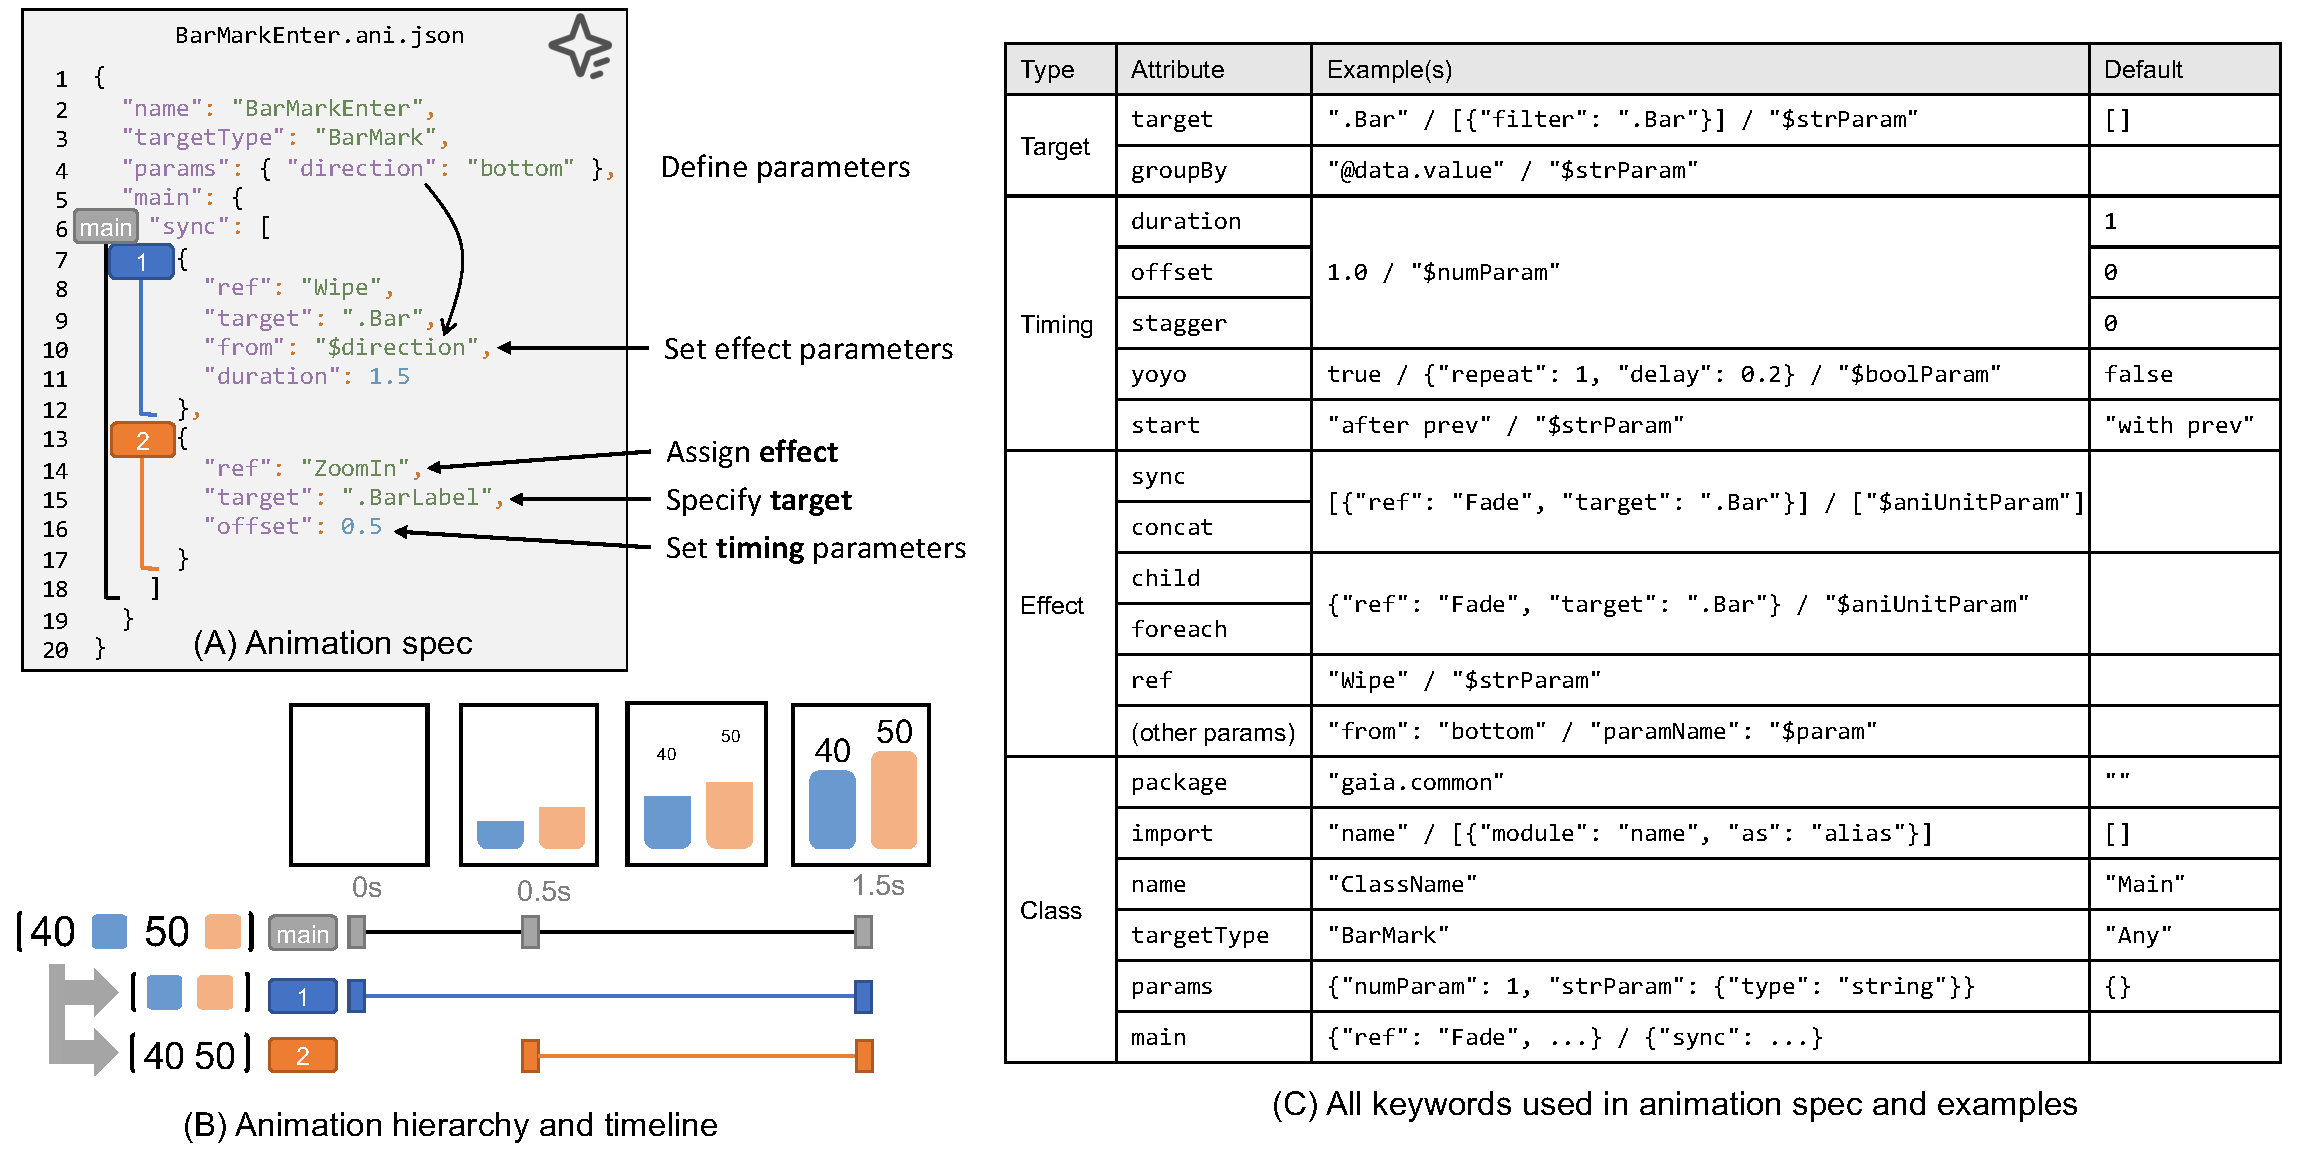
\includegraphics[width=\linewidth]{figs/ani_spec.pdf}
  \caption{
  (A) An example of \gaia{} animation spec, \ie \aniclass{}, designed for BarMark. It contains 3 \aniunit{}s. 
  (B) An animated instance and timeline of the animation created by this spec. \aniunit{}s form a tree hierarchy and each animation selects targets from the parent. 
  (C) All keywords used in \gaia{} animation spec and examples. }
%  \Description{(A) An example of \gaia{} animation spec, \ie \aniclass{}, designed for BarMark. It contains 3 \aniunit{}s. 
%  (B) An animated instance and timeline of the animation created by this spec. \aniunit{}s form a tree hierarchy and each animation selects targets from the parent. 
%  (C) All keywords used in \gaia{} animation spec and examples. }
  \label{fig:ani_spec}
\end{figure}

\aniunit{} describes the effects (using \code{ref}) applied on groups of elements (specifying by \code{target}). 
Formally, one \aniunit{} is an object that contains three types of attributes:
$$
AniUnit := \langle Target, Timing, Effect \rangle
$$
\textit{Target} (\autoref{ssec:gaia_ani_target}) declares the animated target.
Attribute \code{target} defines a list of transforms specifying how an \aniunit{} picks and reshapes targets from its parent.
Attribute \code{groupBy} can only be used with \code{foreach} (introduced in \autoref{ssec:gaia_ani_effect}), grouping the selected elements and applying the effect to each group.
\textit{Timing} (\autoref{ssec:gaia_ani_timing}) contains 4 attributes that describe the common timing settings of an animation.
Attributes of type \textit{Effect} (\autoref{ssec:gaia_ani_effect}) describe how to perform the animation.
One \aniunit{} can refer to an existing effect using \code{ref} (like line 8, 14 in \autoref{fig:ani_spec}(A)).
Especially, \aniunit{} can be nested, using attributes \code{sync}/\code{concat}/\code{foreach}/\code{child} to combine child \aniunit{}s (like \code{sync} animation in \autoref{fig:ani_spec}(A)).
Other animation-related parameters also fall into this category.
\autoref{fig:ani_spec}(C) gives a full list of the attributes and provides some examples.
Strings started with symbol \code{\$} are placeholders for parameters, which will be discussed in \autoref{sec:gaia_reuse}.


\subsection{Target and Target Selection}
\label{ssec:gaia_ani_target}

% Target attribute declared the animated target of \aniunit{}s. 
% Before introducing how target selection works in \gaia{}, we need to formulate the data structure of animated targets.
% As explained by Liu \etal~\cite{liu2018data}, the concept of a collection is defined as a list of elements of the same type, whereas a group can comprise elements of different types.
% Following by the idea of scene graph in Satyanarayan \etal's work~\cite{satyanarayan2015reactive}, \gaia{} abstracts the animated target as a \textbf{tree structure} where leaf nodes are atomic visual elements and internal nodes are groups.
% This abstraction is similar to the SVG structure utilizing \code{g} elements, as shown in \autoref{fig:target}(A).
% Based on this structure, \gaia{} also leverages the W3C Selectors API \cite{eisenberg2014svg} to select the desired targets.

Each \aniunit{} has a \textit{target selection}, which is a \textbf{list of elements}.
It represents the elements that will be animated by this \aniunit{}.
The root selection of an instance is the list containing all visual elements, where each element contains a set of key-value entries as the data (\autoref{fig:target}(A)).

\begin{figure}[h]
  \centering
  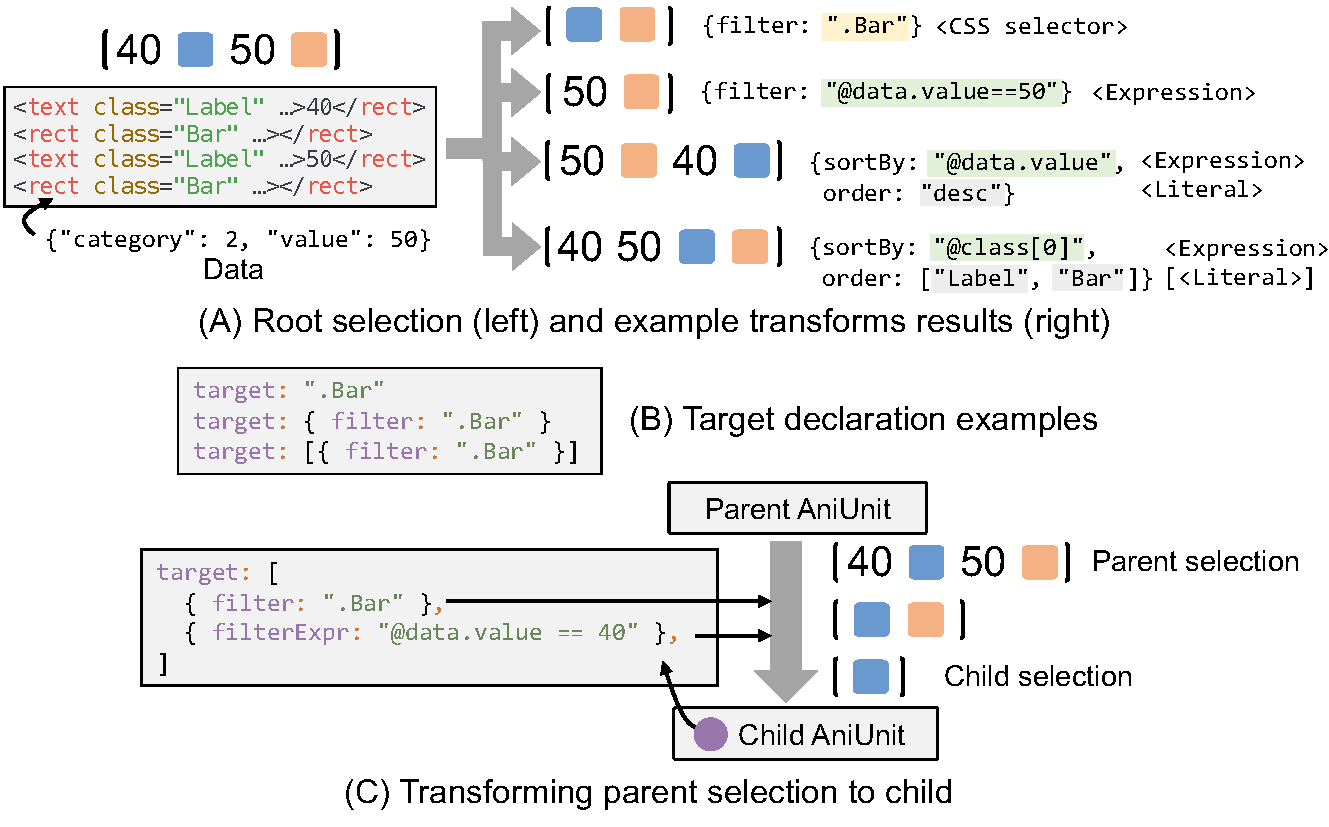
\includegraphics[width=\linewidth]{figs/transform.pdf}
  \caption{
  (A) The root selection of the SVG animated in \autoref{fig:ani_spec}. 
  (B) Examples of transform operations and the corresponding results.
  (C) Properties that can be visited in the expressions.
  (D) Declaring transform operators in attribute \code{target}.
  (E) An example of transforming parent selection to child selection.
  }
%  \Description{
%    (A) The root selection of the SVG animated in \autoref{fig:ani_spec}. 
%    (B) Examples of transform operations and the corresponding results.
%    (C) Properties that can be visited in the expressions.
%    (D) Declaring transform operators in attribute \code{target}.
%    (E) An example of transforming parent selection to child selection.
%  }
  \label{fig:target}
\end{figure}

% Attribute \code{target}, to be specific, declares how to generate target selection from its parent's selection via a sequence of \textit{transform}s.
% We denote the result of transformations as \textit{selection}, which is defined as a collection of groups.
% Intuitively, the selection representing the entire instance (called the root selection) is a collection containing the root group (as shown in \autoref{fig:target}(C)).
% \gaia{} offers four basic types of transform operators, enabling the transformation of one selection into another (\autoref{fig:target}(D-G)):

Attribute \code{target}, to be specific, declares how to generate target selection from its parent's selection via a sequence of \textit{transform}s.
Transform operators in the target attribute are concatenated, working like a pipeline between the parent and child \aniunit{}, allowing users to customize it according to their needs.


\gaia{} offers several basic transform operators, enabling the transformation of one selection into another:

\squishlist

\item \textbf{Filtering}
eliminates all unmatched elements in the collection using either a CSS selector or a predicate expression (two examples are shown in \autoref{fig:target}(B)).

\item \textbf{Sorting}
reorders elements in the collection based on a key expression (two examples are shown in \autoref{fig:target}(B)).
The desired order can be specified using keywords \code{asc} or \code{desc} (only for numerical keys) or by providing a custom list.

\item \textbf{Selecting}
functions similarly to the select and selectAll operator in D3 \cite{bostock2011d3}, querying the descendants within one or multiple groups with a CSS selector.
It allows \gaia{} to process \code{<g>} elements.
%The queries are related to target type structure introduced in \autoref{sec:gaia_reuse}.

% \item \textbf{Grouping}
% organizes groups/elements in the collection into new groups based on a specified key derived from the given expression.

\squishend

Other valid transforms include \textbf{Slicing} (extracting a portion by specifying a start, end, and step) and \textbf{Picking} (selecting one element using index).
The expression will be evaluated during the compilation.
When using expressions, \gaia{} allows users to visit several properties of elements via alias started with symbol \code{@}.
\autoref{fig:target}(C) gives a full list of supported properties.
% In fact, the selection is not performed on the real structure of SVG.
% \gaia{} provides an abstraction layer as introduced in \autoref{sec:gaia_reuse}.

\subsection{Timing}
\label{ssec:gaia_ani_timing}

As listed in \autoref{fig:ani_spec}(C), Timing encompasses 5 attributes: duration, offset, yoyo, stagger, and start.
These attributes govern the timing settings of an \aniunit{}.
Offset is used by the parent animation (\eg sync or concat) to introduce a time delay.
Yoyo enables the implementation of emphasizing animations (\eg blink, highlight, \etcns) by specifying the number of repeats and the delay between each repetition.
Stagger creates animations for each element in the list with an offset compared to the previous one, significantly simplifying "domino effects" as highlighted in \cite{shi2021communicating}.
It can be passed to some basic effect (\eg Wipe) or used with \code{foreach}.
Similar to Canis \cite{ge2020canis}, \code{start} control the reference for staggering in \code{foreach} animation, which can be \code{"with prev"} (start with previous) or \code{"after prev"} (start after previous).

One key consideration for \gaia{}, unlike other techniques, is the application of timing settings (\ie duration) within nested \aniunit{}s.
In \gaia{}, each animation has 4 timing settings: 
(1) inheritance from its parent (\eg a sync animation with a specified duration), 
(2) its own individual settings, 
(3) settings computed from its children (\eg a sync animation consisting of several child animations with set durations) and 
(4) default settings.
\gaia{} prioritizes non-null timing settings in order, and in case of conflicts, it rescales current animations or their children to resolve the conflicts.


\subsection{Effect and Parameters}
\label{ssec:gaia_ani_effect}

Attributes of type \textit{Effect} include all effect-related settings.
In fact, all animation effects can be specified by an animation type identifier along with a set of animation parameters.
For instance, in \autoref{fig:ani_spec}(A), the Wipe animation (lines 7-12) is invoked using the value of \code{ref} with \code{from} serving as the parameter passed to it. 
The parameters can be strings, numbers, boolean, and \aniunit{}s, which provides a flexible way to customize the animation.
For string or number params, users can also use them as a part of other string values, which is useful when defining CSS selectors or expressions to process targets.
As we mentioned above, params can also be used as local variables to prevent declaring several same pieces of spec.
These \aniunit{}s, which include a \code{ref} field, act as the leaf nodes in the animation spec. 
\gaia{} offers a library containing 20+ common animations for different types of elements, such as Fade, Wheel, PathDraw, and more. 
What's more, users can register their own animations in the library and reuse them as needed. 
The library and reusability are the core of \gaia{}, as elaborated further in \autoref{sec:gaia_reuse}.

\begin{figure}[h]
  \centering
  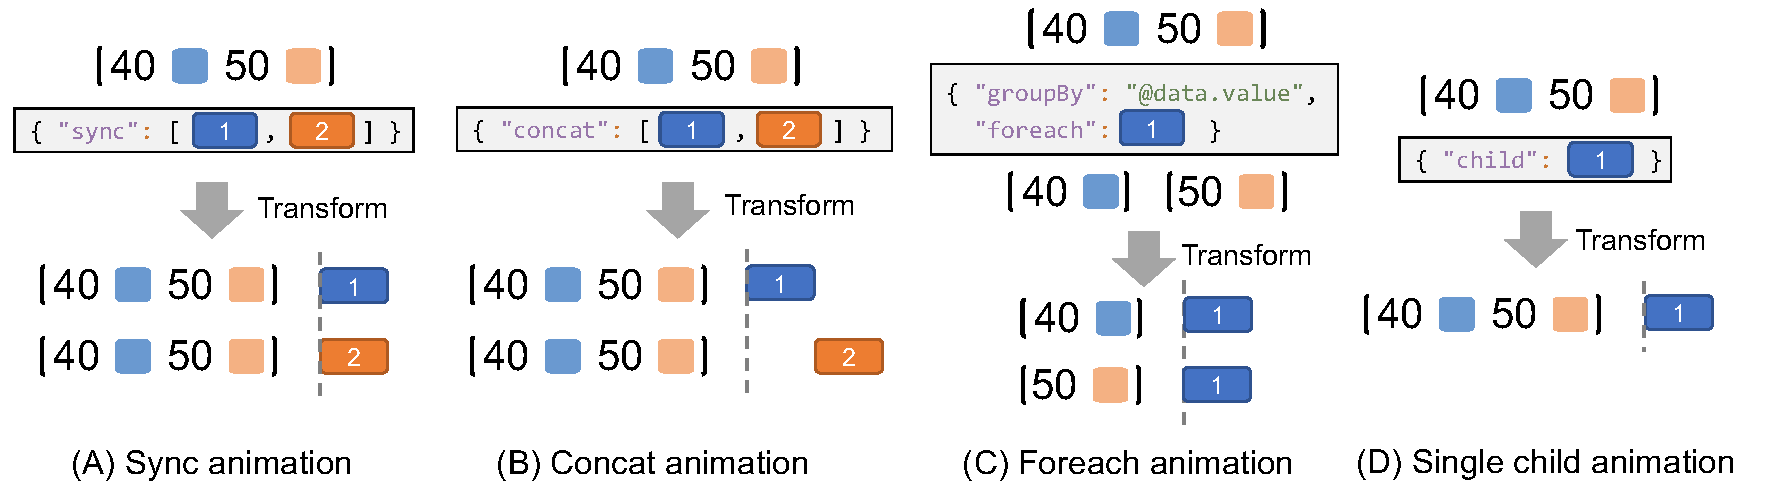
\includegraphics[width=\linewidth]{figs/ani_unit_type.pdf}
  \caption{
    Examples for non-leaf \aniunit{}s (sync, concat, foreach, single-child) in \gaia{}.
  }
%  \Description{Examples for non-leaf \aniunit{}s (sync, concat, foreach, single-child) in \gaia{}.}
  \label{fig:ani_unit_type}
\end{figure}

For non-leaf \aniunit{}s, \eg sync or concat, the children can be treated as one of the parameters as well.
\autoref{fig:ani_unit_type} shows such \aniunit{}s in \gaia{}.
In sync animation, all children are aligned to the start time of this animation.
Concat animation, on the other hand, provides an alternative for building animation hierarchies, where the start time of each child is the end time of the previous one.
In both cases, the \code{"offset"} value defined in the children can further refine the declaration.
In the foreach animation, the elements in the parent selection are first grouped by the value computed by \code{"groupBy"}, and then \gaia{} creates a child animation for each group.
The single-child animation will simply apply the effect on its selection.
It is useful when the inner animation is defined as a parameter.
Except for the foreach animation, all other animations pass the parent selection to the child animation directly with transforming.

\subsection{Tables}

\begin{table}[]
\resizebox{0.5\textwidth}{!}{
\begin{tabular}{|l|l|l|}
\hline
\textbf{Attribute} & \textbf{Example(s)}                                                & \textbf{Default} \\ \hline
\code{target             }& \code{".Bar" / {[}\{"filter":".Bar"\}{]} / "\$strParam"                  }& \code{{[}{]}           }\\ \hline
\code{groupBy            }& \code{"@data.value" / "\$strParam"                                       }& \code{                 }\\ \hline
\code{duration           }& \code{1.0 / "\$numParam"                                                 }& \code{1                }\\ \hline
\code{offset             }& \code{(same as above)                                                    }& \code{0                }\\ \hline
\code{stagger            }& \code{(same as above)                                                    }& \code{0                }\\ \hline
\code{yoyo               }& \code{true / \{"repeat":1,"delay":0.2\} / "\$boolParam"                  }& \code{FALSE            }\\ \hline
\code{start              }& \code{"after prev" / "\$strParam"                                        }& \code{"with prev"      }\\ \hline
\code{sync               }& \code{{[}\{"ref":"Fade","target":".Bar"\}{]} / {[}"\$aniUnitParam"{]}    }& \code{                 }\\ \hline
\code{concat             }& \code{(same as above)                                                    }& \code{                 }\\ \hline
\code{child              }& \code{\{"ref":"Fade","target":".Bar"\} / "\$aniUnitParam"                }& \code{                 }\\ \hline
\code{foreach            }& \code{(same as above)                                                    }& \code{                 }\\ \hline
\code{ref                }& \code{"Wipe" / "\$strParam"                                              }& \code{                 }\\ \hline
\code{(params)           }& \code{"from": "bottom" / "paramName": "\$param"                          }& \code{                 }\\ \hline
\code{package            }& \code{"gaia.common"                                                      }& \code{""               }\\ \hline
\code{import             }& \code{"name" / {[}\{"module":"name","as":"alias"\}{]}                    }& \code{{[}{]}           }\\ \hline
\code{name               }& \code{"ClassName"                                                        }& \code{"Main"           }\\ \hline
\code{targetType         }& \code{"BarMark"                                                          }& \code{"Any"            }\\ \hline
\code{params             }& \code{\{"numParam":1,"strParam":\{"type":"string"\}\}                    }& \code{\{\}             }\\ \hline
\code{main               }& \code{\{"ref":"Fade",...\} / \{"sync":...\}                              }& \code{                 }\\ \hline
\end{tabular}
}
\caption{All attributes}
\end{table}

\begin{table}[]
\resizebox{0.5\textwidth}{!}{
\begin{tabular}{|l|l|l|}
\hline
\textbf{Attribute} & \textbf{Example(s)}                                                & \textbf{Default} \\ \hline
\code{target             }& \code{".Bar" / {[}\{"filter":".Bar"\}{]} / "\$strParam"                  }& \code{{[}{]}           }\\ \hline
\code{groupBy            }& \code{"@data.value" / "\$strParam"                                       }& \code{                 }\\ \hline
\end{tabular}
}
\caption{Target}
\end{table}

\begin{table}[]
\resizebox{0.5\textwidth}{!}{
\begin{tabular}{|l|l|l|}
\hline
\textbf{Attribute} & \textbf{Example(s)}                                                & \textbf{Default} \\ \hline
\code{duration           }& \code{1.0 / "\$numParam"                                                 }& \code{1                }\\ \hline
\code{offset             }& \code{(same as above)                                                    }& \code{0                }\\ \hline
\code{stagger            }& \code{(same as above)                                                    }& \code{0                }\\ \hline
\code{yoyo               }& \code{true / \{"repeat":1,"delay":0.2\} / "\$boolParam"                  }& \code{FALSE            }\\ \hline
\code{start              }& \code{"after prev" / "\$strParam"                                        }& \code{"with prev"      }\\ \hline
\end{tabular}
}
\caption{Timing}
\end{table}

\begin{table}[]
\resizebox{0.5\textwidth}{!}{
\begin{tabular}{|l|l|l|}
\hline
\textbf{Attribute} & \textbf{Example(s)}                                                & \textbf{Default} \\ \hline
\code{sync               }& \code{{[}\{"ref":"Fade","target":".Bar"\}{]} / {[}"\$aniUnitParam"{]}    }& \code{                 }\\ \hline
\code{concat             }& \code{(same as above)                                                    }& \code{                 }\\ \hline
\code{child              }& \code{\{"ref":"Fade","target":".Bar"\} / "\$aniUnitParam"                }& \code{                 }\\ \hline
\code{foreach            }& \code{(same as above)                                                    }& \code{                 }\\ \hline
\code{ref                }& \code{"Wipe" / "\$strParam"                                              }& \code{                 }\\ \hline
\code{(params)           }& \code{"from": "bottom" / "paramName": "\$param"                          }& \code{                 }\\ \hline
\end{tabular}
}
\caption{Effect}
\end{table}

\begin{table}[]
\resizebox{0.5\textwidth}{!}{
\begin{tabular}{|l|l|l|}
\hline
\textbf{Attribute} & \textbf{Example(s)}                                                & \textbf{Default} \\ \hline
\code{package            }& \code{"gaia.common"                                                      }& \code{""               }\\ \hline
\code{import             }& \code{"name" / {[}\{"module":"name","as":"alias"\}{]}                    }& \code{{[}{]}           }\\ \hline
\code{name               }& \code{"ClassName"                                                        }& \code{"Main"           }\\ \hline
\code{targetType         }& \code{"BarMark"                                                          }& \code{"Any"            }\\ \hline
\code{params             }& \code{\{"numParam":1,"strParam":\{"type":"string"\}\}                    }& \code{\{\}             }\\ \hline
\code{main               }& \code{\{"ref":"Fade",...\} / \{"sync":...\}                              }& \code{                 }\\ \hline
\end{tabular}
}
\caption{Template meta}
\end{table}